\documentclass[a4paper,11pt]{article}%Schriftgröße
\usepackage[T1]{fontenc} 
\usepackage[utf8]{inputenc}
\usepackage[german, english]{babel}
\usepackage{graphicx}
\usepackage{ragged2e}
\usepackage[format=plain,
	justification=RaggedRight,
	singlelinecheck=false,
	font={small},labelsep=space]{caption}
\usepackage{xcolor}	
\usepackage[a4paper]{geometry}
	\geometry{left=3.5cm,right=2.5cm,top=2.4cm,bottom=2cm}%Seitenränder
	\usepackage[onehalfspacing]{setspace}%Zeilenabstand
	\renewcommand{\\}{\vspace*{0.5\baselineskip} \newline}
\renewcommand*\MakeUppercase[1]{#1}	
\usepackage{fancyhdr}
	\pagestyle{fancy}
	\renewcommand{\headrulewidth}{0pt}
	\renewcommand{\footrulewidth}{0pt}
	\fancyhead[R]{\footnotesize{\thepage}}
	\fancyhead[L]{\footnotesize{\leftmark}}
	\fancyfoot{}
\usepackage[colorlinks,
	pdfpagelabels,
	pdfstartview = FitH,
	bookmarks = true,
	bookmarksnumbered = true,
	linkcolor = black,
	urlcolor = black,
	plainpages = false,
	hypertexnames = false,
	citecolor = black] {hyperref}



\usepackage[bottom]{footmisc}
\usepackage{amsmath}
\usepackage{amsfonts}
\usepackage{amssymb}
\usepackage{pgfplots}
\pgfplotsset{compat=1.16}
\usepackage{float}
\usepackage{xurl}
\usepackage{booktabs}
\usepackage{caption}
\usepackage{acronym}
\usepackage{nameref}
\usepackage{setspace}
\usepackage{threeparttable}
\usepackage{tabularx}
\usepackage{color,soul}
\usepackage{multirow}
\usepackage{subfigure}

\usepackage{svg}

\usepackage{stackengine}
\usepackage{trfsigns}
\usepackage{bytefield}
%\usepackage[table]{xcolor}
\usepackage{colortbl}

\newcommand{\colorbitbox}[3]{%
         \rlap{\bitbox{#2}{\color{#1}\rule{\width}{\height}}}%
         \bitbox{#2}{#3}}
\definecolor{lightcyan}{rgb}{0.84,1,1}

% settings
\newcolumntype{L}[1]{>{\raggedright\arraybackslash}p{#1}}
\newcolumntype{R}[1]{>{\raggedleft\arraybackslash}p{#1}}
\newcolumntype{C}[1]{>{\centering\arraybackslash}p{#1}}

\newcommand\blfootnote[1]{%
  \begingroup
  \renewcommand\thefootnote{}\footnote{#1}%
  \addtocounter{footnote}{-1}%
  \endgroup
}

% Fußnote linksbündig
\usepackage{scrextend}
\deffootnote[2em]{2em}{1em}{\textsuperscript{\thefootnotemark}\,}

\usepackage{listings}
\usepackage{units}

\definecolor{mGreen}{rgb}{0,0.6,0}
\definecolor{mGray}{rgb}{0.5,0.5,0.5}
\definecolor{mPurple}{rgb}{0.58,0,0.82}
\definecolor{backgroundColour}{rgb}{0.95,0.95,0.92}

\lstdefinestyle{CStyle}{
    backgroundcolor=\color{backgroundColour},   
    commentstyle=\color{mGreen},
    keywordstyle=\color{magenta},
    numberstyle=\tiny\color{mGray},
    stringstyle=\color{mPurple},
    basicstyle=\footnotesize,
    breakatwhitespace=false,         
    breaklines=true,                 
    captionpos=b,                    
    keepspaces=true,                 
    numbers=left,                    
    numbersep=5pt,                  
    showspaces=false,                
    showstringspaces=false,
    showtabs=false,                  
    tabsize=2,
    language=C
}

\graphicspath{
    {pictures/}
}

\begin{document}
\pagenumbering{gobble}
\pagenumbering{roman}

\begin{titlepage}
	\centering
	{\scshape\LARGE TH Köln \par}
	\vspace{1cm}
	{\scshape\Large project report\par}
	\vspace{1.5cm}
	{\huge\bfseries Realizing spatial listening tests in Virtual Reality using Unity\par}
	\vspace{2cm}
	{\Large\itshape Alexander Müller \par}
	\vfill
	Supervised by\par
	M.Sc. Melissa Andrea Ramírez Caro \par \&  \par Prof. Dr. Christoph Pörschmann
	\vfill

% Bottom of the page
	{\large \today\par}
\end{titlepage}


\newpage

\tableofcontents
\newpage

\pagenumbering{arabic}


\section*{Abstract}
\ac{CAPD} is described by the \ac{ASHA} as a condition, which \dq may lead to or be associated with difficulties in higher order language, learning, and communication functions\dq{} without being caused by actual hearing loss or inabilities \cite{ASHA}. Focusing on the aspect of spatial hearing Cameron and Dillon established the term \ac{SPD} and designed the \ac{LiSN} $\&$ Learn auditory training software to improve binaural processing abilities of affected children \cite{LiSN-A}.
\newline
\newline
Based on this foundation a new training software shall be created as an OpenSource project with \ac{VR} support inside the \textit{Unity} game development engine. Apart from offering a free and easy to use alternative to the follow up product of the original program (\textit{Soundstorm) \footnote{Reference: \url{https://www.soundstorm.app/}}} this project shall also evaluate the possible improvements to the concept using the features of an \ac{VR} application. This includes improved immersion into the auditory environment, the support of real 3D-audio in conjunction with head tracking.

\newpage


% What is spatial hearing (short)
% What are the advantages of spatial hearing?
% Obvious: (orientation, reaction to dangers)
% Not so obvious: directive noise filtering, managing noisy environments
% Who has problems: People with hearing inabilities
% Exception:  spatial processing disorder
% Problems of SPD: noisy classrooms and other social events
% LiSN: explanaition of the original paper/study
% What will be done here
\section{Introduction}
\label{sec:introduction}
Spatial hearing describes the ability, to localize the origin of a given sound event, by using binaural clues of the respective signal. The more obvious advantages of this capability include an aid in orientation and improved possibilities to react to events (like an approaching car), which are currently not within the field of view.
\newline
\newline
But apart from this, spatial hearing also allows to separate different sound sources and helps managing noisy environments. This is especially useful if the incoming audio signals are similar to each other. A popular example for this is the \textit{cocktail-party-effect}, which basically described a situation where a listener has to distinguish between a lot of speech signals and focus on a single one in order to be able to maintain a conversation \footnote{For more information refer to \cite{CP}}.
\newline
\newline
Even though this scenario does not cause too much problems for the average person, it contains a lot of difficulties for everyone with hearing inabilities. Unfortunately, in many cases these impairments affect the ability of spatial hearing and therefore reducing or eliminating information that could otherwise be used to separate the different audio sources from each other. Even modern day hearing aids still can't offer the nuances required to precisely determine the location of a given sound source \cite{HA-SRT}.
\newline
\newline
Next to physiological issues causing problems with spatial hearing, it has been found that children with normal hearing thresholds might still not be able to correctly interpret binaural clues. This condition has been associated to \ac{CAPD} and was redefined as \ac{SPD} by Cameron and Dillon in 
\newline
\newline
This effect is described as \ac{SPD}. Since the actual hearing abilities of the affected children is not impaired, they are - in contrast to persons with typical hearing inabilities - provided with all the information required to localize a given sound source. Based on this knowledge the idea was formed, to treat \ac{SPD} by \textit{training} affected children and therefore teaching them, how to correctly interpret binaural clues.
\newline
\newline
Within the \textit{Development and Evaluation of the \ac{LiSN} $\&$ Learn Auditory Training Software for Deficit-Specific Remediation of Binaural Processing Deficits in Children: Preliminary Findings} \cite{LiSN-A} paper by Sharon Cameron and Harvey Dillon it is described how such a training process could look like and already gave some hints \footnote{The original experiments have only been done with a small sample size. Within the conclusion of the paper the requirement of a clinical trial is mentioned, to validate the efficacy of the training process.}.
\newline
\newline
Building upon this approach, the training concept described by Cameron and Dillon shall be transferred into an open-source virtual reality application. This shall bring the additional advantage of combining auditory and visual clues and also allows to further extend the process. 


% Why should anyone rebuild the LiSN software?
% VR advantages
% Extend upon training principle
% Easy access (free)
% OpenSource ideas

% kinda mixed with design principles...




% 1. Test ob so eine Software mit überschaubaren Aufwand in Unity als VR app umgesetzt werden kann
% 2. Wenn ja: Basis für weitere Entwicklungen wie einbezug von Head-Tracking etc. um bessere Training Software bereitzustellen und tiefergehende Forschung zu betreiben (zusammenspiel visuelle und auditorielle Anreize)
% 3. Open-Source: Einbezug verschiedener Entwicklungs- und Adaptierungskompetenz
% 4. Kostenlose Bereitstellung mit wenig Hardware-Anforderungen: weitere Verbreitung solcher Testsoftwares (z.B. auch in Schulen denkbar) und damit bessere Versorgung betroffener Personen
% 5. Option zur Datenerhebung (freiwillig!) -> könnte Forschung weitervorreantreiben...
\section{Motivation}
\label{sec:motivation}
Re-creating the \ac{LiSN} training software as an open-source \ac{VR} application offers several interesting perspectives and possible advantages. The first point would be the option to establish Unity \ac{VR} as a valid foundation for listening related training and test projects. If this can indeed be proven, this project can maybe be used to establish a foundation upon more application can be developed with reasonable resources.
\newline
\newline
The next interesting point would be the evaluation of the additional features that \ac{VR} can bring into this field like head tracking and a more in depth association between auditory and visual clues.
\newline
\newline
Moving on, using an open-source and free-license approach also offers a lot of opportunities. Open-source adds the option that other developers or research teams extend upon the base of this project and in turn help creating a more refined product.
\newline
\newline
Offering the software for free in combination with the - even though not particularly cheap - but rather simple hardware requirements to run such an application, this approach might help improving the availability of such test and training applications for affected persons. If the set-up can be kept simple enough doctors offices, schools or even private households could be able to offer this project.



%Realizing this listening test as a Unity-based \ac{VR} application offers several advantages. The first one being the possibility to implement the project as an OpenSource application. Since only free-to-use assets have been included, both the compiled application and the source files can be made publicly available. Combined with simple setup required to perform the listening experiments, this will hopefully allow a variety of interested groups to perform these tests to collect further data and offer affected children access to work on the condition.
%\newline
%\newline
%Furthermore the Unity framework in conjunction with the prefabs and scripts, that have been created for this project, it would be relatively easy to extend upon the original training concept. For example the addition of multiple distracters within a given scene could very easily be realized.
%\newline
%\newline
%Apart from the previously mentioned aspects the usage VR peripherals for this project also offers a lot more possiblilites. Some of them will be discussed in \Ref{sec:outlook}. But especially adaptive 3D audio in combination with head tracking would allow for a much more realistic scenario. Also the novelty of the VR headset itself will most likely already spark a lot of interest in the participants in comparison to a regular learning/training game.
 

\section{Fundamentals}
\label{sec:fundamentals}
Before describing the general approach of this project in section \ref{sec:approach}, some underlying principles and theoretical foundations shall be discussed. The contents within this section are not supposed to be used as a general explanation but rather as a brief introduction into the topic.

% How do humans localize audio signals
\subsection{Spatial hearing}
In order to localize the source of a given noise, we can use several clues within the perceived sound event. The most important ones being the differences in time and level between the signal on the right and the left ear (Interaul Time/Level Differences [ITD/ILD]). Additionally there are spectral colouring effects, which are based on the path an audio signal takes from it's source, around the listeners head and upper body into the ears. In comparison to ITD/ILDs this effect can only be applied to well known noises, because the listener has to compare the currently perceived noise with previous times in order to identify the spectral differences and assign them to a general direction.   
\newline
\newline
%Auditive localization is based upon the ability to use binaural clues to localize the source of a noise. This ability relies upon three main features: the difference in level (1) and phase (2) of a signal between the left and the right ear and the spectral colouring (3) of a known noise, caused by the geometry of the listeners head and upper body [REFERENCE].
%The human ability of locating audio sources is based upon two main principles
The human ability of locating audio sources can be divided into two main features. The first being the perception of the time and level differences between an acoustic event on the left and right ear. The different time points at which the signal is perceived at the two ears, translates to a different phase at which the audio wave is registered. On the other side the level differences mainly derive from shadowing caused by the head. Both of these effects are not frequency independent, for lower tones the localization via phase differences works better, while at higher frequencies the level variations offer a better indication.
\newline
\newline
The second way of locating a sound source is based upon the spectral differences that occur through the different paths a sound wave can take around the listeners head and upper body. This effect is strongly influenced by the shape of the outer ear, but also the general geometry of the head makes a difference. Basically the head and the ear can be described as directional filters. This kind of localization is mostly based on experiences. The listener can learn to associate the spectral differences in a known noise to the location from which the noise is originated (e.g. by looking for the sound source).

%The actual localization from these perceived spectral differences is based upon previous experience. This means that well known sounds are generally easier to locate, since the listener has more reference data on how a certain kind of noise sounds coming from different directions. However this type of localization is usually more vulnerable towards mistakes. A well known example for this is the so called \dq Front Back Confusion\dq{}.



\subsection{Principles of 3D-audio}
\label{Sec:auralization}
Where auralization focusses on recreating the acoustic properties of a given environment (e.g. a concert hall or a church), ambisonics describes a procedure of recording and playing back a sound field. Both are important foundations for the establishment of authentic \acf{VAE}. 
\newline
\newline
Probably the simplest step towards adding spatial information to audio systems was the move from mono to stereo playback. Nowadays the usage of microphone arrays, extensive speaker setups, \ac{HRTF}s and potent \acs{DSP} systems allows for a much more accurate representation of existing and rendering of virtual auditory scenes.
\newline
\newline
The most common usages of this technologies are most likely surround systems at home or in cinemas and video games. With modern tools it is quite easy to artificially add spatial information to a given noise. To give an example, if a player in a video game shall hear the sound of a door opening behind him, the developers can basically take a \dq dry\dq{} sound (recorded in an acoustically neutral environment) and add reverberation and spatial information later on, depending on the requirements of the scene (distance, size of the room etc.).
%Apart from solely recreating, today's technology can also be used to design \ac{VAE}. By using advanced \ac{DSP} systems and \ac{HRTF}s a noise can freely be located in a free space or even an artificial room and be rendered correctly, so that the listener perceives the source of the signals to be at virtual position. This approach - in a very general way - is used widely to offer \dq surround sound\dq{} or 3D-audio in movies or video games.
\newline
\newline
In the context of \ac{VR} environments this is particularly important, because the user is immersed way deeper into the virtual worlds and inconsistencies between the visual and auditory information associated to a noise would be very noticeable. %Maybe add a reference to this? 




\subsection{Training results}
Before re-working the \ac{LiSN}  project, it is sensible to take a look on the results that could be achieved with the original application. Within \textit{Efficacy of the LiSN \& Learn auditory training software: randomized
blinded controlled study} \cite{LiSN-B} Cameron and Dillon give an insight on the efficacy of the \ac{LiSN-S} training program.
\newline
\newline
Over the course of several studies, it has been proven that auditory training can indeed improve the performance of children affected by \ac{SPD} significantly. Referring to the work of Cameron and Dillon the \ac{LiSN-S} training program achieved an average improvement of the participants of 10.9 dB over the course of 12 weeks. This also supports the data from the initial trials during the development of \ac{LiSN-S}, which found an average improvement of nearly 10 dB over the duration of 3 months \cite{LiSN-A}. However, in both cases - as mentioned by the authors - the sample group was relatively small, so a level of uncertainty remains.
\newline
\newline
Apart from simply performing better within the \ac{LiSN-S} participants showed also improved performances in Fisher's Auditory Performance Checklist\footnote{Reference: \url{http://www.auditorycenter.com/wp-content/uploads/2014/09/APC-Fishers-Auditory-Checklist.pdf}} \cite{LiSN-B}.
\newline
\newline

\section{Approach}
\label{sec:approach}
This section will discuss the basic ideas and prerequisites of this project.


\subsection{Design principles}
Within this section the general design principles and requirements shall be described, before the drafts for how this could be realized will be discussed in section \nameref{sec:concept}.
\newline
\newline
There are three main tasks which shall be used as guidelines for this project:
\begin{enumerate}
\item Re-creating the original software to ensure comparability
\item Only using OpenSource / free license assets to allow for free distribution
\item Create all assets and code segments to be easily adjustable for further extensions
\end{enumerate}

%\subsection{Desing principles}
\paragraph{Comparability} To validate if the new application does actually qualify as a training environment to improve spatial processing abilities, it is sensible to re-create the existing software as close as possible. This would not only allow to compare data from existing research with newly collected data, but also eliminate a lot of effort to check if e.g. the chosen speech stimuli are appropriate for the desired purpose. Additionally if this project does indeed lead to a final application, which could be proven to be a viable alternative, the existing data pools can also be used as reference to evaluate whether extensions (like the addition of head tracking) improves the training effect.


\paragraph{Free distribution} Again assuming the outcome of this project will qualify as a valid training software, the opportunity to be able to make it available as an OpenSource project offers several opportunities. The first one being, that combined with the relatively simple hardware requirements, a free to use software might help improve access to an aid against \ac{SPD} to previously excluded demographics. Additionally a solution, which is more accessible offers the opportunity to gain access to more data, which could be used in further research (e.g. by adding a voluntary option to share progress data within a database). Another aspect would be, that as with any OpenSource project, there is a possibility that other developers or researches use the project as a foundation and extend upon it. This might results in a final product with a widely improved functionality than what would be possible for a single team. However, in any case it is required to only include free to use assets within the implementation to make sure that such a publication won't break any license agreements. So a lot of caution is required when selection third party assets, like sound effects or graphics.


\paragraph{Extensibility} Writing flexible software might be more complicated during the initial development, especially when the scope of the project is rather small. However, to allow the easy addition of new features and simultaneously setting the requirements for a successful OpenSource project, a certain level of flexibility within all parts of the project is necessary. Of course within the given development time frame the extend to that this design principle can be fulfilled is limited, but a lot can be achieved even within the concept phase, if considered and prioritised correctly.


% subseciton{Development tools}
% Unity
% Oculus SDK
% Visual Studio
% Audacity
\paragraph{Development tools} As already mentioned, the major part of the development will be done in Unity with the addition of Visual Studio as \ac{IDE}. The other major tool is the Oculus \ac{VR} \ac{SDK}, which will be used for audio spatialization and of course rendering the visuals to be properly displayed on the given \ac{VR} peripherals.


% free-to-use for non-commercial projects
% graphics and audio rendering is mostly taken care of
% allow great modularbility
% broadly tested and used with a lot of freely available information on how to implement certain features
% at times difficult to handle (not always clear, what's the best way to implement a given feature)
\subsection{Unity overview}
\label{sec:unity}
Unity is a development platform, which is mainly used as a engine for video games. It is free to use for non-commercial, educational or small revenue purposes and therefore qualifies as a foundation for an open-source project \footnote{See \url{https://store.unity.com/\# plans-individual} (retrieval date: November 2021)}. One of the key advantages of using such a framework is that issues like rendering of graphics and audio, portability between different systems etc. are already taken care of. Also Unity includes a wide variety of features, components and available documentation, which significantly speed up the development process. Also the Unity inspector - if used correctly - allows for several ways of adjusting parameters or switching assets without requiring any programming skills. This is especially interesting for this project, since it allows for a low entrance barrier for third parties who want to alter the application in small means to better fit their requirements. However, the vast scope of options given in Unity also adds some drawbacks, like an increased risk of choosing a suboptimal approach when implementing features.

\paragraph{Oculus SDK} The Oculus \acs{SDK} offers a lot of utilities, which make the implementation of a \ac{VR} application a lot easier. This goes from prefabs for camera setups, to input management over the a dedicated audio spatializer.



% describe what parameters will be directly taken from LiSN
\subsection{Orientation on LiSN \& Learn software}
Within this section the given parameters for the training game shall be presented, which have to be followed in order to maintain comparability.
%At this point the fixed parameters from the original training software, which have to be considered to maintain comparability, shall briefly be discussed. 

\begin{itemize}
%\item Adaptive SNR (hit: - 1.5 dB, miss: + 1.5 dB, unsure: + 1.5 dB)
%\item Unsure: Repeat one time with increased SNR
%\item practice rounds (min 5 with 3 dB steps to find SRT of participant)
\item Word list (List 1)
%\item Reward system (5 consecutive correct guesses)
%\item Four word options for each guess
%\item Session length (40 rounds)
%\item 2 Speakers (male, female)
%\item 2 groups (with or without spatial information (90 deg target/dist offset)
%\item Given RMS levels of target (-22 dB) and distracter (-25 dB)
\item Target sentence generation (cutting sentences into words, then randomly assembling them)
\end{itemize}

% \subsection{Training Game}
\paragraph{Game loop} Like in the original project the main game loop will consist of target sentences being playing along with a distracter story. After every round \textbf{4 options} for a word from the target sentence and an \textit{Unsure} button will be presented to the player. A training session consists of 40 rounds / sentences.

\paragraph{Scenarios} The training game shall feature \textbf{4 different scenarios}:
\begin{enumerate}
\item Same voice with 0 degrees (low cue \ac{SRT})
\item Same voice with $\pm$ 90 degrees (high cue \ac{SRT})
\item Different voices with 0 degrees (low cue \ac{SRT})
\item Different voices with $\pm$ 90 degrees (high cue \ac{SRT})
\end{enumerate}
For this purpose both all the target sentences and distracter stories have to be available with two differnt voices (ideally a female and a male one).

\paragraph{Unsure} If the player selects \textit{Unsure} the same sentence will be repeated once. If \textit{Unsure} is selected a second time, a new sentence will be played.

\paragraph{Adaptive SNR} Based upon whether the participant guess a word correctly (\textit{hit}), incorrectly (\textit{miss)} or select the \textit{unsure} option the audio levels between target and distracter will be adjusted:
\begin{itemize}
\item Hit: - 1.5 dB SNR
\item Miss: + 2.5 dB SNR
\item Unsure: + 1.5 dB SNR
\end{itemize}

\paragraph{Practice mode} To find the \ac{SRT} of the participant, a \textit{practice mode} will be started at each session, where the given answers are not included in the progress data. A minimum of \textbf{5 practice rounds} have to be done before starting the actual training game. Once this minimum has been reached the first incorrect or \textit{Unsure} selection will end \textit{practice mode}. During \textit{practice mode} the \ac{SNR} decreases by 3 dB.

\paragraph{Rewards} When \textbf{5 consecutive correct answers} have been given, the participant is granted a reward sticker, which will be shown on the screen for the remaining duration of the session.

\paragraph{Sound feedback} On every \textit{hit} or \textit{miss} either a \dq success\dq{} or \dq failure\dq{} has to be played.

\paragraph{Attention sound} 500 ms before the start of every target sentence a short attention sound has to be played (1000 Hz tone of 200 ms).

\paragraph{Playback delays} The disctracter story shall always start 2 s before the target sentences and end approx. 1s after the target speaker has finished.

\paragraph{Audio parameters} Each target sentence shall be normalized to -22.0 dB \acs{RMS}. Every distracter story has to be normalized to - 25.0 dB \acs{RMS}.

% \subsubsection{Audio assets}

% voice options
% RMS for distractor and target
% audio editing guidelines

%\subsection{Audio assets}
%\label{sec:audio_assets}
%As basis for this project the word lists given in the appendix of the LiSN paper \cite{lins} are used. Since due to the huge variety of options, the only feasible way to construct the sentences is by assembling a sentence through seperate audio files for each word. This however comes with a problem. Simply recording single words and then playing the files one after another strongly alter the speech flow and accentuation, which would normally be present when the sentence is spoken.
%\newline
%\newline
%To handle this problem, the words won't be recorded separately but instead a subset of the possible sentences from each list will be recorded. Within this subset all words from the list are included within the recordings. Afterwards the recorded sentences will be cut into the individual words and then will be used the assemble randomly generated sequences based on these assets. This should work fine, since the structure of all sentences within any list remains the same. So the speech flow and pronunciation between the sentences should not be too larger. GET SOME REFERENCES FOR THIS ASSUMPTION!
%\newline
%\newline
%It also has to be considered that of course the phonetic differences between a given word group will also differ. So in some cases it might be a lot easier for a listener to guess the correct word, since some options of the given selection can be excluded, even if the correct word wasn't fully understood.


\subsection{Visuals}
\label{sec:visuals}
Apart from the move to \ac{VR} peripherals and the new audio assets the visuals will probably be the biggest deviation from the original software. Since the 2D presentation of the \ac{LiSN} software wouldn't be sensible here, a 3D environment has to be added.
\newline
\newline
Considering that the target participants of this project are children the visual presentation is of great importance. If the training game isn't engaging, there is a high risk of participants not complying with the required training schedule due to the repetitive nature of the sessions\footnote{This issue was already brought up by Cameron and Dillon in the conclusion of \cite{LiSN-B}}.
\newline
\newline
The novelty of \ac{VR} in general might already be helpful in mitigating this problem, but it should still be considered during development. Additionally \ac{VR} applications require special care when it comes the orientation and sense of space within the 3D environment, otherwise there is a risk of players feeling disorientated.
\newline
\newline
Due to the limited resources in this development, the usage of 3rd-party assets will most likely be inevitable. To still be able to freely distribute the project the license requirement for all non-proprietary assets has to be considered.


\paragraph{Matching visuals to audio} Since in the original context neither reflections nor reverberation was included, it shouldn't be added in the re-modelling as well. This adds some conditions to the selection of the 3D environment. A big empty room, would suggest the occurrence of reverb and echo and should therefore be avoided. Ideally an outside location should be selected, where a free-field sound propagation would be natural. Another important point would be the visual representation of the speakers. Since it might be distracting to here a voice from a given direction without being able to associated the sound to any object in the world, the addition of \textit{avatars} for the speakers should be considered.


%\paragraph{Avatars} Another important part is the graphical representation of the audio sources. Since we have the visual component given through the \ac{VR} headset, the sound should not simply come from an invisible sources, but have a origin which the user can identify through the graphics. This however includes another challenge. Of course it would be possible to create humanoid avatars with complex animations - including lip syncing - to convey that the object is indeed active and not just a passive talking rock. However this would take a huge amount of effort to pull of. Instead a different path will be used here, which is also pretty common in budget oriented game design (e.g. indie games). Through abstract avatars and simple animations/movements it is possible to convince the user, that the object is alive and active, while at the same time requiring a lot less effort to pull of.


%\subsubsection{Audio Sources}
%Within the level both interactive and regular audio sources are implemented. All of them use 3D rendering, so that the preceived sound changes based on the position of the player to the object, emitting the sound. The advantage of adding interactive sound sources is that,...

% Tatsächliche Testumgebung mit Datenerfassung
% 4 Optionen: 0/90 deb, same/different voice
% 4 Listen, zufällige Sätze, 4 Rate Optionen
% Audio parameter (SNR zwischen Talker/Distractor)
% Welche Daten werden erfasst: Totals, Hits, Misses, List, Group (?)
% Wie/Wann wird zwischen Wordgruppen gewechselt?
%\subsection{Training-Game}
%\label{sec:training_game}


%\subsubsection{Audio files}
%Target sentences are constructed in a way that the co-articulation in between the sentences of a list is similar enough the allow randomly scrambling up sentences will maintaining a natural sounding result.

%\subsubsection{Game loop}
%Continuous distracter stories creating a noise with similar characteristics as the target sentences.
%\newline
%\newline
%Both the target sentences and the distracter stories shall be omitted by actual objects within the game world. This association between audio and visual representation shall create further immersion (FIND REFERENCE!).
%\newline
%\newline
%Whenever a target sentence was played, four word options will be displayed. (IMAGES OR WORDS?). When the correct result is picked, the selected option turns green and a celebratory sound is played. Otherwise if an incorrect option is selected, it is marked red and a failure sound is played. Alternatively an  \dq uncertain\dq{} option is presented.
%\newline
%\newline
%SNR: For every correct guess, the SNR is decreased by 2.5 dB. For every incorrect guess, SNR is increased by 1.5 dB. At uncertain at first the same sentence is repeated with 1.5 dB higher SNR. At a second consecutive \textit{uncertain} a new sentence will be played, with again increased SNR.


\section{Concept}
\label{sec:concept}
While section \ref{sec:approach} only described the general design principles and foundations of the application, this section shall be used to discuss how these requirements  actually be fulfilled and which parts of the project might cause issues.
\newline
\newline
The biggest part will be achieving flexibility in the projects structure, to allow other users to adapt the application to their requirements.


\subsection{Training Game}
This section will focus on the aspects that are specific to the actual training game. This includes some pre-considerations on how the general setup should look like and what practices can be used to maintain a certain level of adjustability from the start. Of course it is to be expected, that some of the ideas described here won't be implemented exactly.

\subsubsection{Audio Sources}
Inside the training game there will be two possible setup option for the audio sources. In \textbf{Setup A} the \textit{target} audio source will be placed directly in front of the \textit{main camera}, while the \textit{distracter} will be moved 90 degrees to the right side \footnote{The selection between right and left side is arbitrary. Interchanging both options during or between sessions would also be an option.}. In \textbf{Setup B} both audio sources will be placed directly in front of the \textit{main camera} and therefore no spatial information can be used to differentiate both audio streams. In both options the distance of the sources to the \textit{main camera} hjas to be the same.
%\vspace{5mm}
\begin{figure}[h!]
	\hspace{0.1\textwidth}
    \subfigure[Setup A]{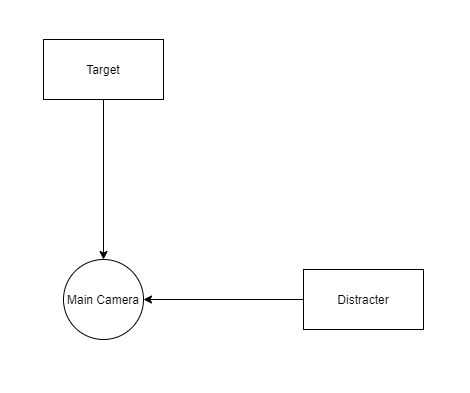
\includegraphics[width=0.4\textwidth]{trainingSetupPageA.png}}
    %\hspace{0.2\textwidth}
    \subfigure[Setup B]{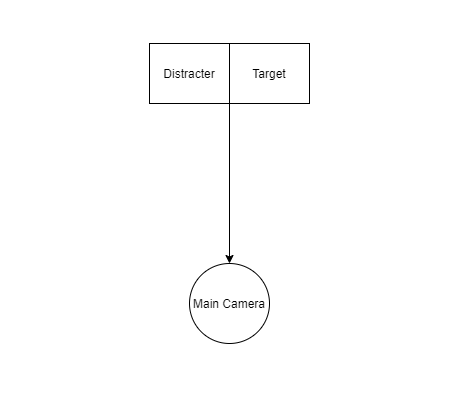
\includegraphics[width=0.4\textwidth]{trainingSetupPageB.png}}
    %\hspace{0.1\textwidth}
\caption{Training Game Setup}
\label{fig:setups}
\vspace{3mm}
\end{figure}
\newline
%\vspace{8cm}
\newline

\subsubsection{Word databases}
Even though the initial scope of the application shall only feature a single word list from the original paper (Appendix A \cite{LiSN-A}), the implementation should be flexible enough to support different word databases. This is particularly important when considering the option to port the application to different languages. To further elaborate on how this should be done, List 1 from the original paper will be used as an example.  Within table \ref{tab:list1} all highlighted words are can be used as an \textit{option} to question the user.
\begin{table}[h!]
\begin{tabular}{|p{2cm}|p{2cm}|p{2cm}|p{2cm}|p{2cm}|p{2cm}|}
\hline
& Subject & Verb & Count & Adjective & Objects \\
\hline
The & \textbf{baby} & bought & \textbf{two} & big & \textbf{apples} \\
\cline{2-6}
 & \textbf{boy} & carried & \textbf{three} & blue & \textbf{bottles} \\
\cline{2-6}
 & \textbf{clown} & cleaned & \textbf{four} & borken & \textbf{cars} \\
\cline{2-6}
 & \textbf{doctor} & drew & \textbf{five} & green & \textbf{chairs} \\
\cline{2-6}
 & \textbf{girl} & dropped & \textbf{six} & little & \textbf{crayons} \\
\cline{2-6}
 & \textbf{lady} & had & \textbf{seven} & old & \textbf{cups} \\
\cline{2-6}
 & \textbf{man} & liked & \textbf{eight} & orange & \textbf{shoes} \\
\cline{2-6}
 & \textbf{nurse} & saw & \textbf{nine} & red & \textbf{spoons} \\
\cline{2-6}
 & \textbf{teacher} & watched & \textbf{ten} & yellow & \textbf{trucks} \\
\hline
\end{tabular}
\caption{LiSN - List 1}
\label{tab:list1}
\end{table}
\vspace{5mm}
When observing this table three parameters can be determined:
\begin{itemize}
\item Sentences length: \textbf{6 words}
\item Possibilities for each group: \textbf{9 options}
\item Number of 'selectable' groups: \textbf{3 selectable groups}
\end{itemize}
\vspace{5mm}
Of course this could be extended even further, like adding sentences of variable length or alternating the 'selectable groups'. But as with many of these decisions, offering too many options might lead to problems (e.g. the generated sentences won't be as comparable if they are allow to differ in length).
\newline
\newline
All three of these parameters have to be considered when creating a dynamic framework, which shall be able to support different word lists. Of course it 
\newline
Additionally this example also provides and interesting anomaly. All \textit{options} within a given \textit{group} are sorted alphabetically, except the \textbf{Count} - words. It is important to not rely on any order in which the list might be created, or any other parameter that depends on the actual content of a given word list.
\newline
\newline
Issues like co-articulation effects have to be considered by the creator of a given group.


\subsection{Asset management}
\label{sec:asset_management}
Moving on from the requirement of establishing a framework, which supports variable \textit{word database} formats the topic of how assets can be added or changed within the application has to be considered.
\newline
\newline
Unity offers multiple ways to handle this topic. The straight forward approach would be to assign the individual asset files through drag and drop within the inspector. Even though this would in principle fulfil the requirement of changing/adding assets, it's not ideal when many assets shall be changed at once (consider List 1 (table \ref{tab:list1}, where already 9 x 5 audio files for the individual words would have to be added manually). 
\newline
\newline
Instead the \textit{Resource} system shall be used to handle this group of assets. This offers the opportunity to load assets straight from the file system into the application. However this solution also has some drawbacks. At first the path of the assets within the file system has to be considered. Once option would be to enforce a main path with naming policies. A path could then look like this: \textit{Resources/Audio/WordList<\textbf{number}>/Group<\textbf{number}>}.


\subsection{Progress tracking}
In order for this application to be useful, an option has to be added to track the progress of the user over the course of multiple training sessions. At first it has to be defined, which information has to be tracked in order receive all required data to not only monitor possible improvements of a single user but also to compare the results of multiple participants against each other within the context of a study.
\newline
\newline
The most obvious parameter to be tracked would be the \ac{SRT}. In order to recognize a progress this has to be stored for each training session. It would of course also be possible to not only keep the average \ac{SRT} value of each sessions, but also the \ac{SNR}s of each individual sentences combined with the information if the guess was \textit{correct}, \textit{incorrect} or \textit{unsure}. However, even though both the target and distracter audio assets have been normalized there might still be some fluctuations within the perceived sound levels of both sources, which can't be tracked or even noise from outside of the application. Therefore this data would come with several uncertainties and is also not required if the data evaluation shall be done in comparison to the original paper.
\newline
\newline
Another important part would be to allow for differentiation between regular participants of a study and a control group. Therefore a \textbf{group} parameter should also be added.


\paragraph{User System} Another part which has to be considered, is the option that more than one person might use the same system to do training sessions. To make sure that the progress can be tracked individually, a user system shall be established. Within this system access to the \textit{training game} shall be restricted via a typical login screen requiring the correct \textbf{username} and \textbf{password} to be entered. Adding new users should also be possible from the login screen, where \textbf{username} and \textbf{password} can freely be set (as long as the username isn't already in use). Within the 'user creation' progress the already mentioned differentiation between regular and control group could also be added and be linked to the user account.


\paragraph{Progress export} Next to tracking the progress data for each user, it should also be made accessible from outside of the application in a format that allows easy evaluation with external tools. For this purpose all user data shall be stored within a \textit{.json} file. This allows to hold multiple types of data from \textit{strings} for the username to arrays of \textit{floats} for the \ac{SRT} values and easily readable as well as widely used in many different applications.


\paragraph{In-app visualization} Finally to application shall give any user an option to keep track of their progress. This will be realized through a separate screen, which features a simple graph plotting the \ac{SRT} values of the amount of traning sessions done as well as additional space to show e.g. the current average \ac{SRT} over all sessions.


\subsection{User interface}
\label{sec:ui-concept}
Based on the previously described parts of the application, a general setup for the required \ac{UI} options can be defined. At first it is important, that all \ac{UI} elements can easily be selected while using \ac{VR} peripherals. This could for example be achieved by setting an appropriate minimal size for all text that displayed. Since a lot of this 
\newline
\newline
Apart from this general consideration, a brief overview of all major \ac{UI} elements shall be given


\paragraph{Main Menu} The \textit{Main Menu} only requires button to access different screens (e.g. \textit{Training Game} or \textit{Progress}).

\paragraph{Login} This requires of course text fields which can be used to type down both the username and password. Additionally a \textit{Submit} and a \textit{Create new user} button are necessary.

\paragraph{User Creation} This can basically be the same as the \textit{Login Screen}, with the addition that the user has to select a group (control or regular) to be associated with the account.

\paragraph{Progress} As already described, the \textit{Progress} screen shall display a combination of different information. As interactive object a \textit{Return} button has to be added, to allow the user to return to the \textit{Main Menu}.

\vspace{5mm}
\begin{figure}[h!]
\centering
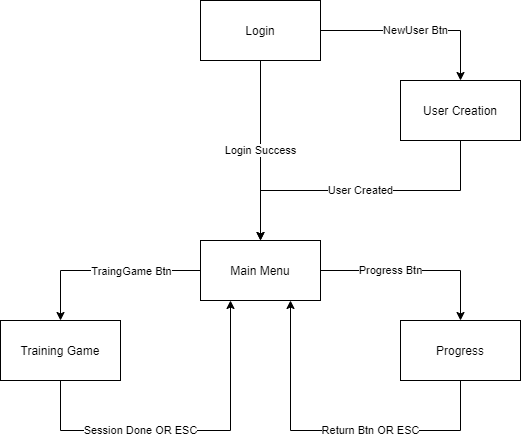
\includegraphics[width=0.7\textwidth]{screens2.png}
caption{Screens}
\label{fig:screens}
\vspace{3mm}
\end{figure}



% Progress
% TG: Voice Selection
% TG: Word Selection
\section{Conclusion}
\label{sec:conclusion}
Within part A of this research project, a concept as well as the main set of requirements for recreating the \ac{LiSN} software has been presented. Of course as within every software development process it is to be expected that some parts of the final product will derive from the initial concept, due to either new insights into the subject matter or unforeseen difficulties during the implementation.



\newpage
\section*{Abbreviations}
\vspace{5mm}
\begin{acronym}[SEVENLTH]
 \acro{ASHA}{American Speech-Language-Hearing Association}
 \acro{CAPD}{Central Auditory Processing Disorder}
 \acro{GUI}{Graphical User Interface}
 \acro{HRTF}{Head Related Transfer Function}
 \acro{IDE}{Integrated Development Environment}
 \acro{LiSN}{Listening in Spatialized Noise \& Learn}
 \acro{LiSN-S}{Listening in Spatialized Noise - Sentences Test}
 \acro{RMS}{Root Mean Square}
 \acro{SDK}{Software Development Kit}
 \acro{SNR}{Signal to Noise Ratio}
 \acro{SPD}{Spatial Processing Disorder}
 \acro{SRT}{Speech Reception Threshold}
 \acro{UI}{User Interface}
 \acro{VAE}{Virtual Acoustic Environments}
 \acro{VR}{Virtual Reality}
\end{acronym}

\newpage
\listoffigures
\addcontentsline{toc}{section}{List of Figures}
%\newpage
\renewcommand\refname{Sources}
\addcontentsline{toc}{section}{Sources}
\begin{thebibliography}{14}
\bibitem{ASHA}{\textit{Central Auditory Processing Disorder}, \acf{ASHA}, retrieval date: Nov. 2021, \url{https://www.asha.org/Practice-Portal/Clinical-Topics/Central-Auditory-Processing-Disorder/}}
\bibitem{LiSN-Dev}{\textit{Development and Evaluation of the Listening in Spatialized Noise Test}, Sharon Cameron, Harvey Dillon, Date: March 2006, \url{https://www.researchgate.net/publication/7326536_Development_and_Evaluation_of_the_Listening_in_Spatialized_Noise_Test}}
\bibitem{LiSN-A}{\textit{Development and Evaluation of the LiSN $\&$ Learn Auditory Training Software for Deficit-Specific Remediation of Binaural Processing Deficits in Children: Preliminary Findings}, Sharon Cameron, Harvey Dillon, Date: November 2011, \url{https://www.researchgate.net/publication/51975813_Development_and_Evaluation_of_the_LiSN_Learn_Auditory_Training_Software_for_Deficit-Specific_Remediation_of_Binaural_Processing_Deficits_in_Children_Preliminary_Findings}}
\bibitem{LiSN-B}{\textit{Efficacy of the LiSN \& Learn auditory training software: randomized
blinded controlled study}, Sharon Cameron, Helen Glyde and Harvey Dillon, Date: October 2015, \url{https://www.researchgate.net/publication/276222698_Efficacy_of_the_LiSN_Learn_auditory_training_software_Randomized_blinded_control_study}}
%\bibitem{LiSN-C}{\textit{Correlating performance on the Listening in Spatialized Noise – Sentences Test (LiSN-S) with the Listening in Spatialized Noise – Universal Test (LiSN-U)}, Kiri Mealingsa, Sharon Cameron and Harvey Dillon, Published: April 2020, Date: 2019}
\bibitem{CP}{The cocktail-party problem revisited: early processing and selection of multi-talker speech, Adelbert W. Bronkhosrt, Date: April 2015, \url{https://www.researchgate.net/publication/274397643_The_cocktail-party_problem_revisited_early_processing_and_selection_of_multi-talker_speech}}
\bibitem{HA-SRT}{\textit{Listening through hearing aids affects spatial perception and speech intelligibility in normal-hearing listeners}, Jens Cubick, Jörg M Buchholz, Virginia Best, Mathieu Lavandier, Torsten Dau, Date: 2016, \url{https://www.ncbi.nlm.nih.gov/pmc/articles/PMC6246072/}}
%\bibitem{test}{test \href{https://www.google.com/}{This link is colored blue.}}
% Add Unity and Oculus references...

\end{thebibliography}

\end{document}